% vim: set spell spelllang=es syntax=tex :

\section{Fútbol de robots}

\label{mt_futbolRobots}

La \emph{RoboCup} \cite{robocupHist} (del inglés \emph{Robot World Cup}) es una
competencia internacional celebrada desde 1997, donde equipos de robots juegan
una versión simplificada del fútbol. Su finalidad es la de ofrecer un ambiente
controlado donde poner a prueba los avances en distintas áreas de conocimiento
como la inteligencia artificial, visión por computadora y robótica. Existen
cinco ligas distintas cuyas características varían desde la simulación del
ambiente y robots, hasta robots humanoides con visión local:

\begin{description}

	\item[Liga simulada:] Tanto los robots como el ambiente son simulados.
		El movimiento de cada robot es controlado por un agente de
		software independiente y con visión local. El sistema de
		simulación tiene información precisa de la posición y
		orientación de todos los robots y la pelota en la cancha
		virtual, pero la información entregada a los agentes de software
		es con ruido, y relativa a su posición y orientación.

		Está compuesta de dos sub-ligas, la liga simulada
		bidimensional y la liga simulada tridimensional.

	\item[Liga de tamaño pequeño:] También llamada \emph{SSL}, del inglés
		\emph{Small Size League}, es la liga más antigua de la
		\emph{RoboCup}. Cada equipo controla sus robots a través de un
		sistema centralizado. La visión es global y compartida por ambos
		equipos. Las cámaras están montadas sobre la cancha en
		posiciones fijas, y cada robot es identificado por parches en su
		parte superior. Los parches están diseñados para poder ser
		identificados rápidamente. Debido a la posición de las cámaras y
		los parches, son observables completamente en toda la cancha.
		Los robots se mueven sobre ruedas y tienen un ``pie'' para
		patear la pelota.

	\item[Liga de tamaño mediano:] En ésta los robots tienen visión local
		y son agentes independientes. Al igual que la liga pequeña, se
		mueven sobre ruedas y tienen un ``pie'' para patear la pelota.

	\item[Plataforma estándar:] Esta liga introduce un modelo de robot
		estándar sobre el cual todos los equipos deben ejecutar su
		software. En la actualidad se utiliza el robot \emph{NAO} de
		\emph{SoftBank Robotics}, un robot humanoide. La visión es
		local y cada robot es autónomo, pero pueden comunicarse.

	\item[Liga humanoide:] En esta liga los robots intentan simular
		características humanas, no sólo en su forma, sino también en
		las limitaciones sensoriales y su autonomía.

\end{description}

Debido a la simplicidad del sistema de visión global de la \emph{SSL} y la
necesidad de que este sistema responda en tiempos acotados, consideramos que el
sistema resulta útil para introducir a los alumnos a los temas de visión por
computadora y aplicaciones paralelas.

Un partido de la \emph{SSL} enfrenta a dos equipos de seis robots, que deben
tener un tamaño menor que un cilindro de 9$cm$ de radio y 15$cm$ de alto
\cite{sslrules2015}, se movilizan sobre ruedas y tienen un ``pie'' con el que
patear la pelota. Los detalles de su construcción no están reglamentados,
aunque los equipos suelen coincidir en algunos puntos, como por ejemplo el uso
de ruedas omnidireccionales.

Cada equipo cuenta con una computadora fuera del campo de juego, a la cual se
delega la toma de decisiones y planeamiento del movimiento de los robots. Por
su parte la capacidad de procesamiento de los robots se limita a aquella
necesaria para ejecutar las órdenes de movimiento de la computadora de su
equipo. Estas computadoras perciben el ambiente a través de un sistema de
visión global centralizado compartido. Se utiliza un conjunto de cámaras,
montadas sobre distintas áreas del campo de juego y conectadas a una
computadora donde se ejecuta el sistema de visión. El sistema detecta la
posición y orientación de cada uno de los robots y la posición de la pelota, y
reporta esta información a las computadoras que controlan los equipos.

Para que el sistema de visión pueda identificar a cada robot, cada uno tiene
sobre su parte superior cinco parches de colores. El parche que se encuentra en
el centro indica el color del equipo del robot, y los cuatro restantes sirven
para identificar al robot dentro del equipo y para conocer su orientación en
cada momento. La pelota es de un color uniforme y distinto al de los parches de
los robots; normalmente, naranja, ya que este color contrasta fácilmente con el
verde de la cancha. En la figura \ref{sistemaVG} se muestra la arquitectura del
sistema con tres robots, dos del equipo azul y uno del equipo rojo.

\begin{figure}[!htb]

	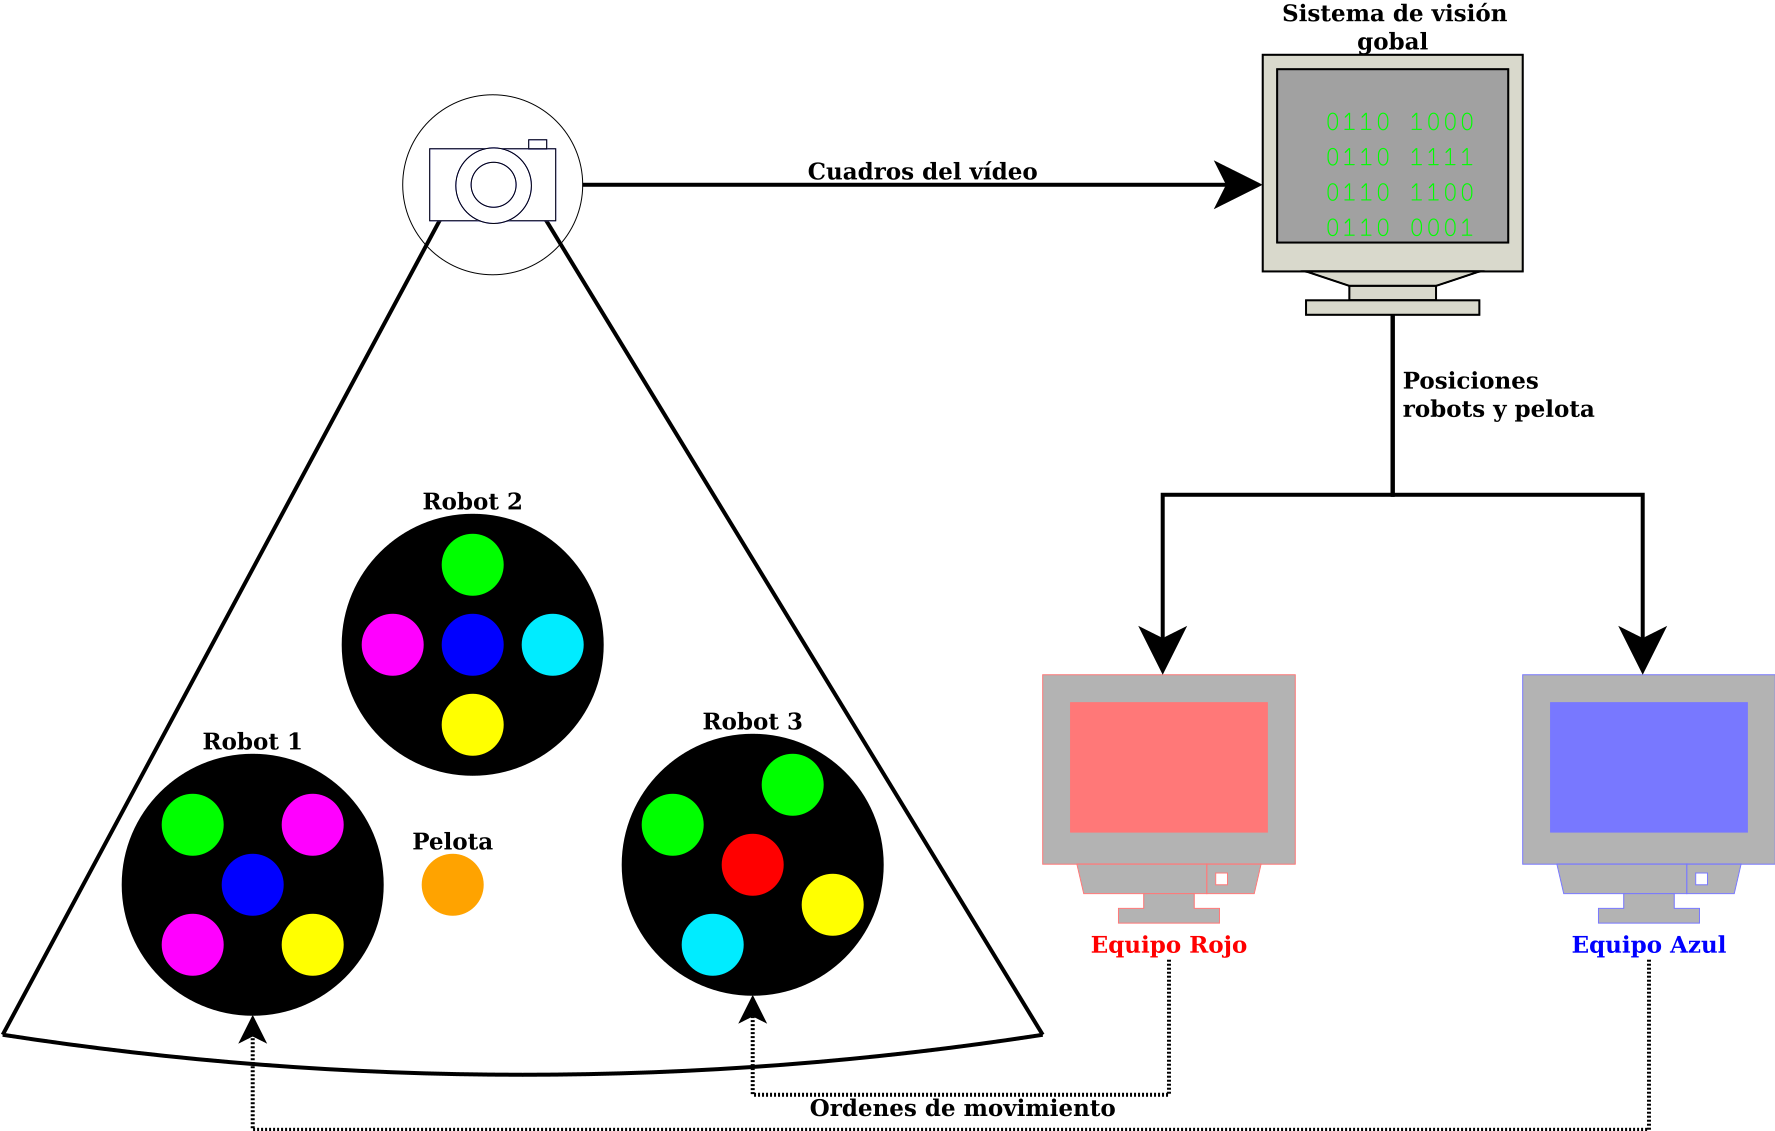
\includegraphics[width=\textwidth]{img/sistemaVG.pdf}

	\caption{Estructura de comunicación del sistema de visión global en
	fútbol de robots de la \emph{SSL}.}

	\label{sistemaVG}

\end{figure}

El uso de este sistema centralizado permite a los participantes abstraerse de
los problemas de la visión por computadora y enfocarse en la estrategia del
juego. Además, permite que las tareas de calibración y montaje de las cámaras se
realicen una sola vez para cada campo de juego, en vez de para cada partido.

Las computadoras utilizadas para la ejecución del sistema de visión global son
equipos de escritorio de gama media o alta. Esto permite que el sistema pueda
ser ejecutado en el sitio donde se lleva a cabo el partido de la \emph{SSL} y
aumenta la cantidad de equipos de hardware disponibles.

El fútbol de robots se desarrolla en un contexto de tiempo real, ya que el
ciclo completo de procesamiento de información debe cumplirse en un plazo
máximo para poder alcanzar los objetivos. El servidor debe procesar cada
cuadro para entregar la información de posición y orientación de cada elemento
en el campo de juego a las computadoras coordinadoras de los equipos; y éstas
deben tomar una decisión y comunicarla a los robots, todo dentro de un tiempo
de respuesta razonable para el progreso de la aplicación.

Los parámetros de calidad de este tipo de sistema son, normalmente:

\begin{itemize}

	\item 	taza de aciertos en la detección de objetos;

	\item 	precisión en la posición y orientación de los aciertos en la
		detección de objetos;

	\item 	precisión en la posición y orientación de los robots y pelota;

	\item 	cuadros por segundo (\emph{FPS}, del inglés \emph{Frames Per
		Second}) procesados;

	\item 	y máximo tiempo de espera del cuadro (tiempo desde la creación
		del cuadro hasta la entrega de la información extraída).

\end{itemize}

Originalmente el tamaño de la cancha era de 4,9$m\times$3,4$m$, lo que permitía
que todo el campo de juego fuera observado con una sola cámara. Luego se optó
por dos tipos de canchas en los partidos de la \emph{SSL}: las canchas de tamaño
simple, con un tamaño de 6,05$m\times$4,05$m$ para las cuales se utilizan dos
cámaras, una sobre cada media cancha, y las de tamaño doble, con un tamaño de
8,09$m\times$6,05$m$, que utilizan cuatro cámaras, una por cada mitad de cada
media cancha. En la figura \ref{cancha} se muestran los tamaños de las canchas y
la distribución de las cámaras.

\begin{figure}[!htb]

	\centering

	\begin{subfigure}[!htb]{0.45\textwidth}
		\centering
		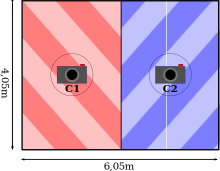
\includegraphics[scale=0.8]{img/cancha605cm.pdf}
		\caption{}
	\end{subfigure}
	~
	\begin{subfigure}[!htb]{0.45\textwidth}
		\centering
		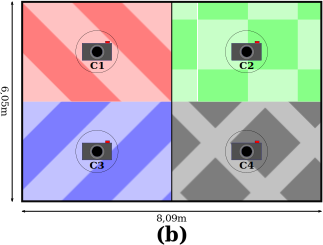
\includegraphics[scale=0.8]{img/cancha809cm.pdf}
		\caption{}
	\end{subfigure}

	\caption{Dimensiones y área de cobertura de las cámaras en la liga
	\emph{SSL}, en competencias a) anteriores a 2015; b) año 2015 y
	posteriores.}

	\label{cancha}

\end{figure}

Desde el año 2015, las canchas de tamaño doble son las utilizadas de forma
predeterminada \cite{sslrules2015}. Con este cambio se espera permitir la
exploración de nuevas tácticas por parte de los equipos, ya que una mayor área
de juego permite a los robots movimientos de mayor amplitud y variedad.

Sin embargo, como consecuencia, en las canchas de tamaño doble, el sistema de
visión debe procesar cuatro veces más información que en las canchas
originales y el doble que las canchas de tamaño doble, lo que da lugar a un
problema para un sistema de tiempo real como éste. El aumento en la cantidad
de información impacta negativamente en el rendimiento debido a que se reducen
los cuadros por segundo procesados y se incrementa el tiempo de espera del
cuadro.

Como se utilizan computadoras de escritorio convencionales para la ejecución
del sistema de visión global es sensato asumir que se trata de un sistema de
memoria compartida de múltiples núcleos, pero el sistema actual utilizado por la
\emph{SSL} ejecuta en un solo hilo, aprovechando sólo uno de los núcleos
disponibles.

Para poder entregar la información requerida en tiempos acotados utilizando sólo
un hilo de ejecución, los plugins del sistema están altamente optimizados. Esto
tiene como efecto colateral que el sistema no es ideal para ser utilizado como
herramienta didáctica para la introducción a la visión por computadora, ya que
cada plugin que se agregue o modifique deberá ser optimizado para que el sistema
mantenga su rendimiento.
